\section{Results}
\label{ch:results}
\noindent	

This chapter intends to present the results of the project.

\subsection{Matrix sandbox}

\begin{figure}[H]
	\begin{center}
		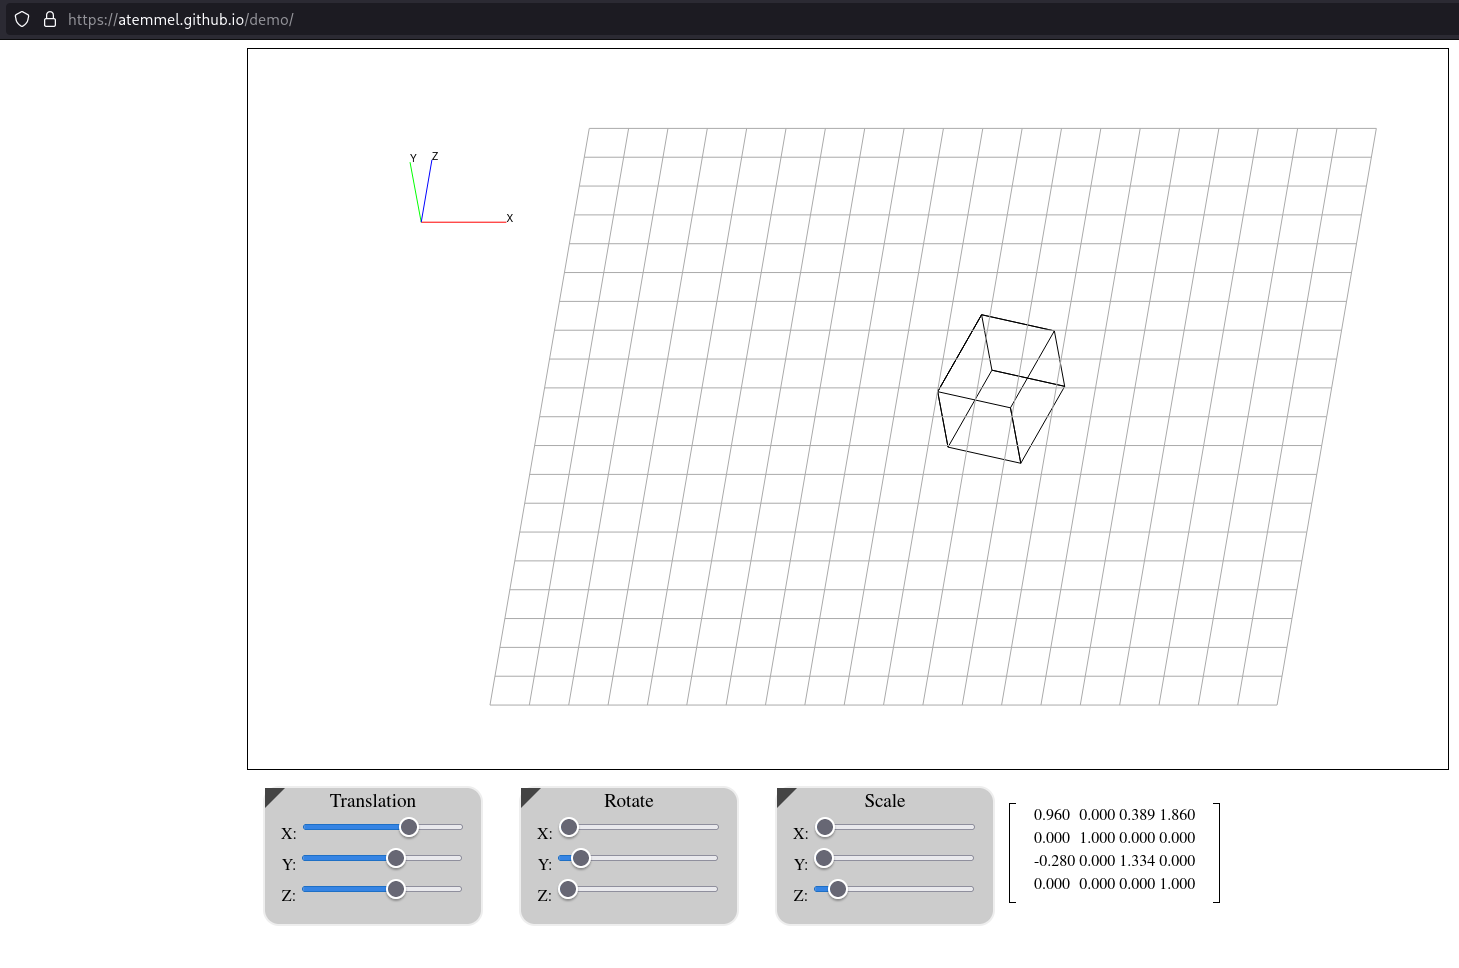
\includegraphics[width=\textwidth]{./img/matrix_sandbox.png}
		\caption{Screenshot taken from the matrix sandbox.}
		\label{matsand}
	\end{center}
\end{figure}

The matrix sandbox is presented in \textit{figure~\ref{matsand}} as an interactive website in which users are able to explore the possibilities of presenting transforms using matrices. The majority of the website shows a cube and a grid as well as a coordinate frame for the purpose of orienting the user. Also present is a set boxes containing sliders which represent individual properties that the different transformation matrices hold. These boxes can be rearranged by dragging and dropping them, resulting in new sets of transformations depending on the order that they are presented in. Lastly, the end transformation is visualized as a 4x4 matrix, allowing users to directly see the consequences of their transformations.

\subsection{Raytracer}

\begin{figure}[H]
	\begin{center}
		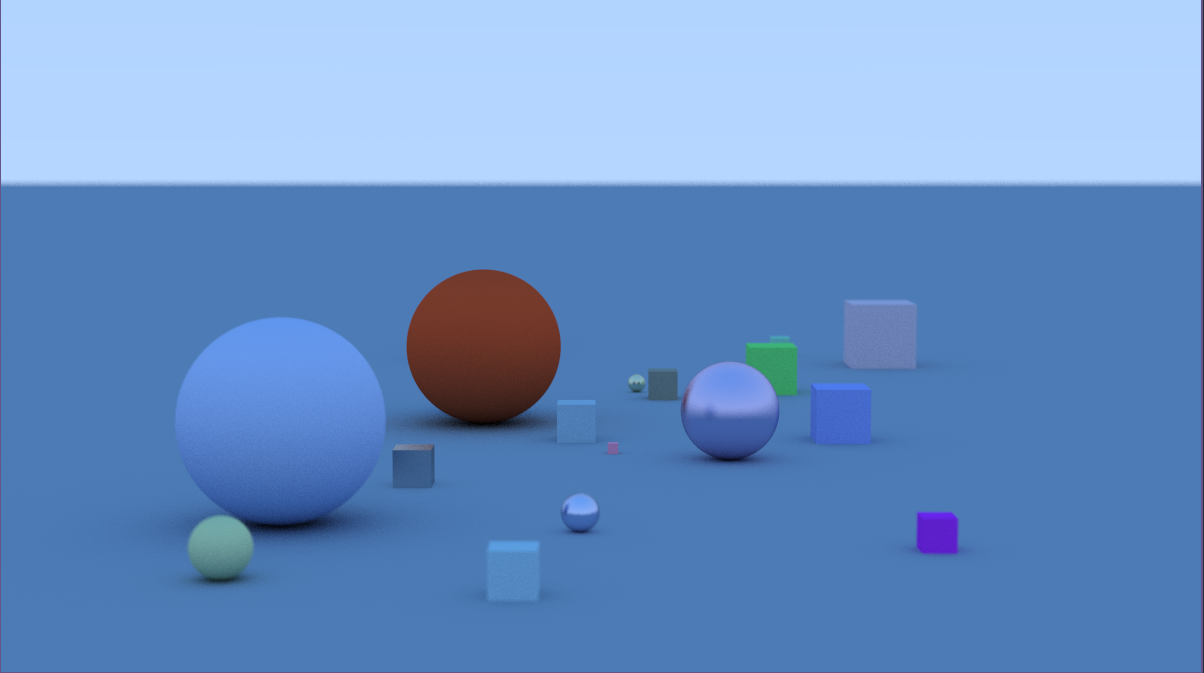
\includegraphics[width=\textwidth]{./img/dunder_bild.png}
		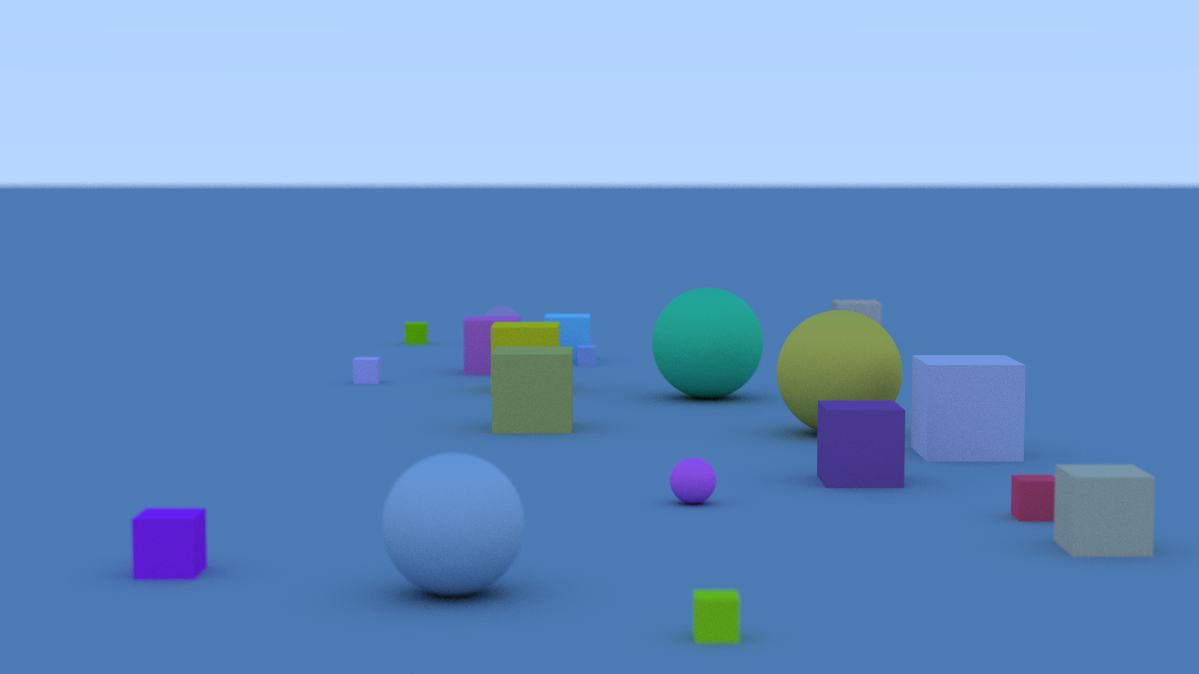
\includegraphics[width=\textwidth]{./img/pog_bild.png}
		\caption{Screenshots taken from the raytracer.}
		\label{matsand}
	\end{center}
\end{figure}
	
The raytracer was also finalized, with features such as:

\begin{itemize}
	\item Support for rendering of spheres and boxes.
	\item Support for lambertian and metallic materials.
	\item Multithreaded rendering.
	\item Basic depth-of-field effect.
\end{itemize}

Before the rendering starts, positions, dimensions and materials of several shapes are randomized, leading to each invocation of the raytracing producing a result that is likely to be completely different from the invocation before.

\iffalse
The results chapter is included when you have produced a systematic study, i.e. an evaluation of a program that you have developed, which is required for C - and D-level diploma work. In the results chapter objective results of the empirical study are presented. Keep in mind that possible comments in this chapter should only be used for clarification. Your own views and subjective (personal) comments belong in the chapter conclusion/discussion.

Strive to present the results, for example measurement-, calculations- and/or the simulation result, in a form that is as lucid and easily understandable as possible. The results are preferably presented in diagrams or tables. Accounts of interviews can be summarised, but may include concrete examples supporting your work.

Extensive results, for example complete summaries of survey results, large tables and long mathematical deductions, are placed in the appendices.
\fi
